\subsection{Results of Experiments}
The experimentation aims to compare the facial recognition capabilties of both
PCA and autoencoder approaches. Hence the experiments consists of two parts.
First, the extracted features of both methods performed on the Yale Face
Database B will be compared. Finally, these diagnostic features' class
recognition ability will be checked in numerical experiments. In the case of
PCA, a support vector machine (SVM) is used for classification. The experiments
have been conducted using sci-kitlearn \cite{sk} library in Python. I
have adapted Facebook DeepFace model implementation from
\cite{serengil2017tensorflow101}, which uses Keras \cite{chollet2015keras} and
Tensorflow \cite{tensorflow2015-whitepaper} as its backend. In the autoencoder's
case, the extracted feautres will be forwarded to a softmax classifier,
consisting of one fully-connected layer and softmax activation function with 38,
accounting the amount of classes.

\begin{figure}[h]
  \begin{subfigure}{}
    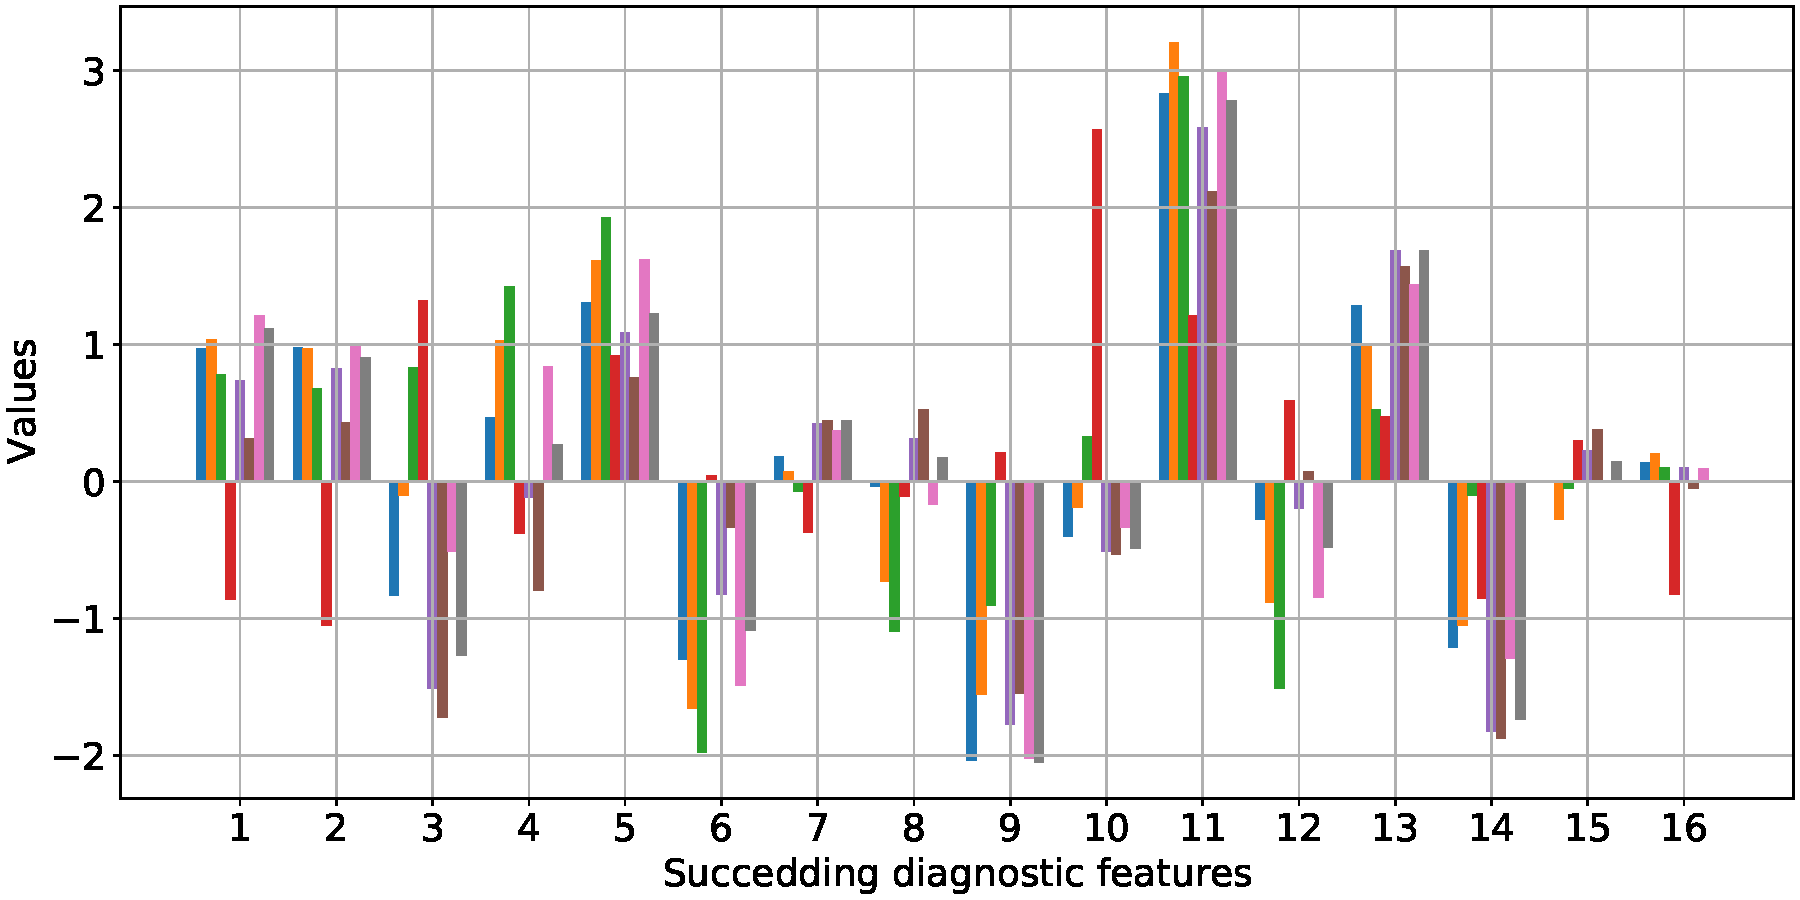
\includegraphics[width=\columnwidth]{PCAfeatures.pdf}
  \end{subfigure}

  \begin{subfigure}{}
    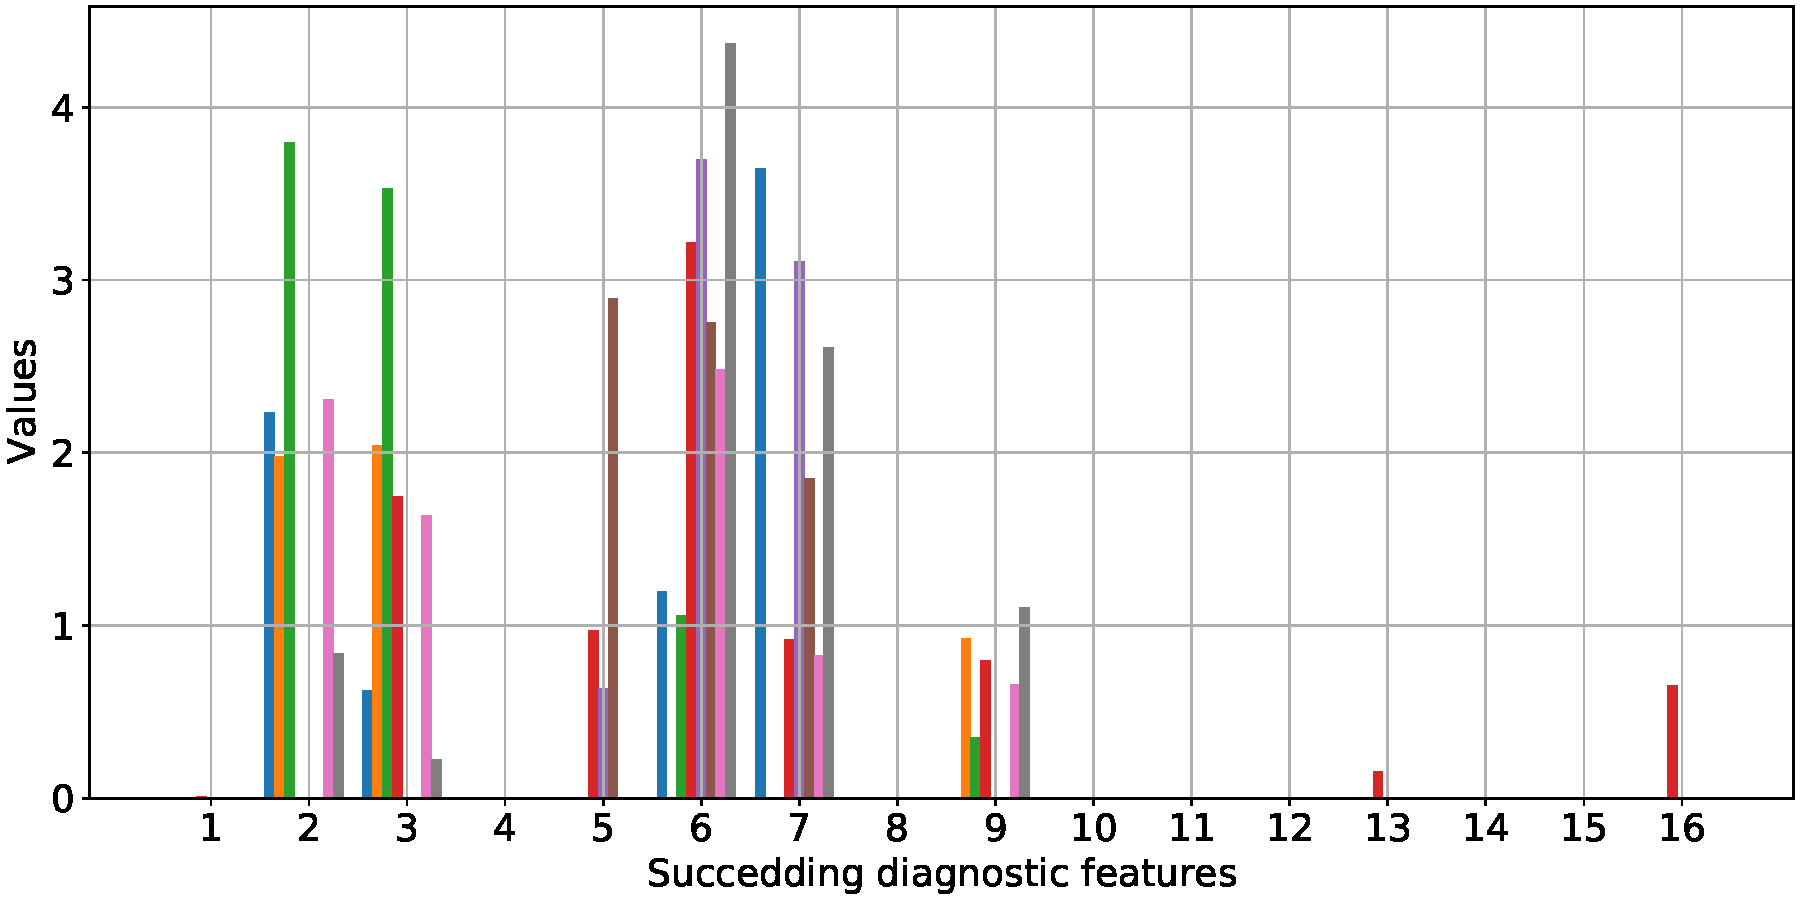
\includegraphics[width=\columnwidth]{Encoderfeatures.pdf}
  \end{subfigure}

  \caption{The diagnostic feature representation of 8 different images of the same person: (above) the distribution of PCA feautes (below) the corresponding features created by an autoencoder}
  \label{features}
\end{figure}

While the face library is decomposed into 150 principal components for PCA, the
amount of features generated by the DeepFace model is 4096 as described in
section \ref{sec:deepFace}. Fig. \ref{features} illustrates the representation
of the first 16 features extracted by the two methods respectively. All of them
correspond to eight different images of the same person. 

The key to successful face recognition is insesitivity of the extracted features
to different poses and lighting conditions of the face. The autoencoding
principle to feature generation is very efficient in this respect. This is seen
well in Fig. \ref{features}: the activations of PCA features fluctuate a lot.
Values are positive and negative for the same person, resulting in a high
standard deviation of the feature distribution. In contrast, the features
computed by the autoencoder are around the same level for the same person. Note
that because only the first 16 features are shown, some signals are not or not
fully activated. Similar results are found in \cite{siwek2017autoencoder}, where
the authors show that autoencoders find better balanced discriminant features.
The different quality of encodings generated by the two approaches, can be
caused through the inherent limits, resulting from PCA only being a linear
transformation. Autoencoders on the other hand introduce various
non-linearities, enabling it to find discriminant features a PCA simply cannot.
However, the autoencoder's transformation in a ''latent space`` are rather non
intuitive and thus function more like a black box. As illustrated in Fig.
\ref{eigenfaces}, the calculated principal componets on the other hand have
intuitive interpretations as eigenfaces, while these are ordered by their
statistical significance.

For face classification on the Yale Face Database, it was split at random choice
of learning and testing data, while maintaining 38 classes present in both
respectively. 60\% of samples have been used in learning and 40\% in testing. In
the case of PCA, the classifier used is a SVM with Gaussian kernel. The width of
Gaussian function and regularization constant C have been adjusted using
\textit{GridSearchCV} using a standard 5=fold cross validation applied on the
training set. Their optimal values found in experiments were as follows $C=1000$
and $\gamma=0.01$. In the case of the autoencoder, the softmax classifier was
trained for 50 epochs during each the model's performance was validated on the
crossentropy loss and weights optimized with ADAM.

\begin{table}[h]
  \caption{The average accuracy of face recognition for 38 classes of data (persons) obtained at application of autoencoder and pca preprocessing}
  \begin{center}
  \begin{tabular}{|c|c|c|}
  \hline
  \textbf{Metric} & \textbf{PCA} & \textbf{Autoencoder} \\
  \hline
  Accuracy & 92.60\%$\pm$0.99\% & \\
  \hline
  \end{tabular}
  \label{scores}
  \end{center}
\end{table}
